\makeatletter
\providecommand{\bigsqcap}{%
  \mathop{%
    \mathpalette\@updown\bigsqcup
  }%
}
\newcommand*{\@updown}[2]{%
  \rotatebox[origin=c]{180}{$\m@th#1#2$}%
}
\makeatother

\chapter{Design}
\label{chapter:Design}


\section{COUNT Policy}
\label{section:countpolicy}

\begin{wrapfigure}{r}{0pt}
\resizebox{0.4\textwidth}{!}{

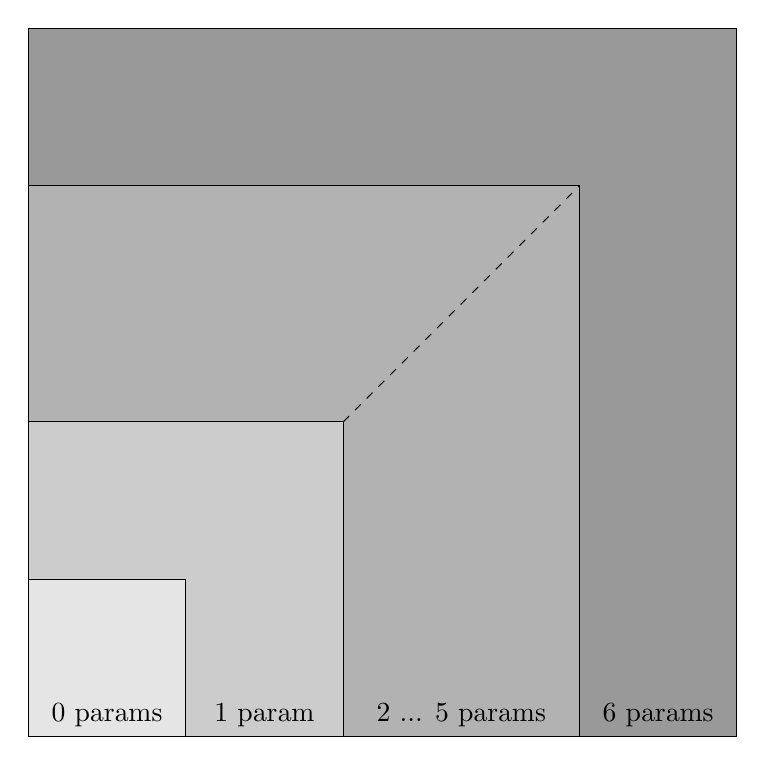
\begin{tikzpicture}


\fill[black!40!white] (0,0) rectangle (9,9);
\fill[black!30!white] (0,0) rectangle (7,7);
\fill[black!20!white] (0,0) rectangle (4,4);
\fill[black!10!white] (0,0) rectangle (2,2);


\draw (0,0) --node[anchor=south] {0 params} (2,0)  -- (2,2) -- (0,2) -- (0,0) ;

\draw (0,0) -- (2,0) --node[anchor=south] {1 param} (4,0) -- (4,4) -- (0,4) -- (0,0);


\draw (0,0) --(4,0) --node[anchor=south] {2 ... 5 params} (7,0) -- (7,7) -- (0,7) -- (0,0);

\draw (0,0) --(7,0) --node[anchor=south] {6 params} (9,0) -- (9,9) -- (0,9) -- (0,0);

\draw[dashed] (4,4) -- (7,7);
	
\end{tikzpicture}

}
\caption{COUNT policy schema}
\label{fig:COUNTschema}
\end{wrapfigure}

What we call the COUNT policy is essentially the policy introduced by typearmor\cite{typearmor}. The basic idea revolves aroung classifying calltargets by the number of parameters they provide and callsites by the number of paramters they require. Furthermore, generating 100\% precise measurements for such classification with binaries as the only source of information is rather difficult. Therefore overestimations of parameter count for callsites and underestimations of the parameter count for calltargets is deemed acceptable. This classification is based on the general purpose registers that the call convention of the current ABI - in this case the SystemV ABI - designates as parameter registers. Furthermore, we completely ignore floating point registers or multiinteger registers. The core of the COUNT policy is now to allow any callsite $cs$, which provides $c_{cs}$ parameters, to call any calltarget $ct$, which requires $c_{ct}$ parameters, iff $c_{ct} \leq c_{cs}$ holds. However, the main problem is that while there is a significant restriction of calltargets for the lower callsites, the restriction capability drops rather rapidly when reaching higher parameter counts, with callsites that use 6 or more parameters being able to call all possible calltargets:
\[
	\forall cs_1, cs_2.  c_{cs_1} \leq c_{cs_2} \Longrightarrow  \| \{ct \in \mathcal{F} | c_{ct} \leq c_{cs_1} \} \| \leq \| \{ct \in \mathcal{F} | c_{ct} \leq c_{cs_2}  \} \|
\]
One possible remedy would be the ability to introduce an upper bound for the classification deviation of parameter counts, however as of now, this does not seem feasible with current technology. Another possibility would be the overall reduction of callsites, which can access the same set of calltargets, a route we will explore within this work.




\section{TYPE Policy}
\label{section:typepolicy}

\begin{wrapfigure}{r}{0pt}
\resizebox{0.5\textwidth}{!}{
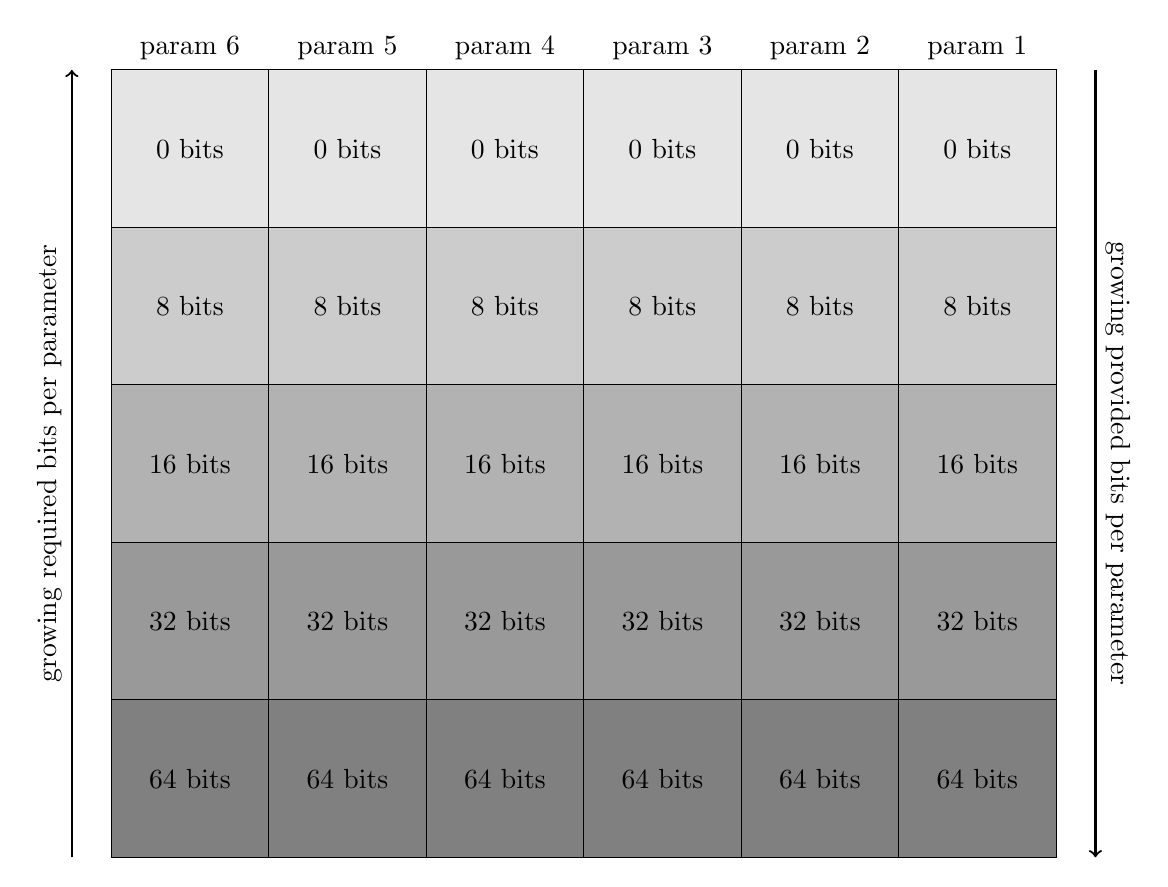
\begin{tikzpicture}

\fill[black!10!white] (0,10) rectangle (12,8);
\fill[black!20!white] (0,8) rectangle (12,6);
\fill[black!30!white] (0,6) rectangle (12,4);
\fill[black!40!white] (0,4) rectangle (12,2);
\fill[black!50!white] (0,2) rectangle (12,0);

\draw[thick,->] (-0.5,0) -- node[sloped, anchor=center, above] {growing required bits per parameter} (-0.5,10);
\draw[thick,->] (12.5,10) -- node[sloped, anchor=center, above] {growing provided bits per parameter} (12.5,0);

\draw (0,10) --node[anchor=south] {param 6} (2,10);
\draw (2,10) --node[anchor=south] {param 5} (4,10);
\draw (4,10) --node[anchor=south] {param 4} (6,10);
\draw (6,10) --node[anchor=south] {param 3} (8,10);
\draw (8,10) --node[anchor=south] {param 2} (10,10);
\draw (10,10) --node[anchor=south] {param 1} (12,10);

\draw (0,10) rectangle node[anchor=center] {0 bits} (2,8);
\draw (2,10) rectangle node[anchor=center] {0 bits} (4,8);
\draw (4,10) rectangle node[anchor=center] {0 bits} (6,8);
\draw (6,10) rectangle node[anchor=center] {0 bits} (8,8);
\draw (8,10) rectangle node[anchor=center] {0 bits} (10,8);
\draw (10,10) rectangle node[anchor=center] {0 bits} (12,8);

\draw (0,8) rectangle node[anchor=center] {8 bits} (2,6);
\draw (2,8) rectangle node[anchor=center] {8 bits} (4,6);
\draw (4,8) rectangle node[anchor=center] {8 bits} (6,6);
\draw (6,8) rectangle node[anchor=center] {8 bits} (8,6);
\draw (8,8) rectangle node[anchor=center] {8 bits} (10,6);
\draw (10,8) rectangle node[anchor=center] {8 bits} (12,6);

\draw (0,6) rectangle node[anchor=center] {16 bits} (2,4);
\draw (2,6) rectangle node[anchor=center] {16 bits} (4,4);
\draw (4,6) rectangle node[anchor=center] {16 bits} (6,4);
\draw (6,6) rectangle node[anchor=center] {16 bits} (8,4);
\draw (8,6) rectangle node[anchor=center] {16 bits} (10,4);
\draw (10,6) rectangle node[anchor=center] {16 bits} (12,4);

\draw (0,4) rectangle node[anchor=center] {32 bits} (2,2);
\draw (2,4) rectangle node[anchor=center] {32 bits} (4,2);
\draw (4,4) rectangle node[anchor=center] {32 bits} (6,2);
\draw (6,4) rectangle node[anchor=center] {32 bits} (8,2);
\draw (8,4) rectangle node[anchor=center] {32 bits} (10,2);
\draw (10,4) rectangle node[anchor=center] {32 bits} (12,2);

\draw (0,2) rectangle node[anchor=center] {64 bits} (2,0);
\draw (2,2) rectangle node[anchor=center] {64 bits} (4,0);
\draw (4,2) rectangle node[anchor=center] {64 bits} (6,0);
\draw (6,2) rectangle node[anchor=center] {64 bits} (8,0);
\draw (8,2) rectangle node[anchor=center] {64 bits} (10,0);
\draw (10,2) rectangle node[anchor=center] {64 bits} (12,0);
\end{tikzpicture}
}

\caption{TYPE policy schema for callsites and calltargets}
\label{fig:TYPEschema}
\end{wrapfigure}
What we call the TYPE policy is the idea of not only relying on the parameter count but also on the type of a parameter. However due to complexity reasons, we are restricting ourselves to the general purpose registers, which the SystemV ABI designates as parameter registers.
These are 64bit registers that can be accessed in 4 different ways:
\begin{itemize}
\item the whole 64bits of the register
\item the lower 32bits of the register
\item the lower 16bits of the register
\item teh lower 8bits of the register
\end{itemize}
Four of those registers can also directly access the higher 8bits of the lower 16bits of the register. For our purpose we register this access as a 16bit access. Based on this information, we can assign a register one of 5 possible types $\mathcal{T} = \{64, 32, 16, 8, 0\}$. We also included the type 0 to model the absence of data within a register. Similar to the COUNT policy, we allow overestimation of types in callsites and underestimation of types in calltargets. However, the matching idea is different, because as can we depict in Figure \ref{fig:TYPEschema}, the type of a calltarget and a callsite no longer depends solely on its parameter count, each callsite and calltarget has its type from the set of $\mathcal{T}^6$, with the following comparison operator:
\[
	u \leq_{type} v :\Longleftrightarrow  \forall_{i = 0}^{5} {u_i \leq v_i} , \text {with } u, v \in \mathcal{T}^6
\]
Again we allow any callsite $cs$ call any calltarget $ct$, when it fulfillst the requirement $ct \leq cs$. The way we represent this is by letting the type for a calltarget parameter progress from 64bit to 0bit - If a calltarget requires a 32bit value in its 1st parameter, it also should accept a 64bit value from its callsite - and similarly we let the type for a callsite progress from 0bit to 64bit - If a callsite provides a 32bit value in its 1st parameter it also provides a 16bit, 8bit and 0bit to a calltarget. Now the advantage of the TYPE policy in comparison to the COUNT policy is that while our type comparison implies the count comparison, the other direction does not hold. Meaning, just having an equal or lesser number of parameters than a callsite, does no longer allow a calltarget being called there, thus restricting the number of calltargets per callsite even further. A function that requires 64bit in its first parameter, and 0bit in all other parameters, would have been callable by a callsite providing 8bit in its first and second parameter when using the COUNT policy, however in the TYPE policy this is no longer possible.


\section{Instruction Analysis}
\label{section:instructionanalysis}
Usually dataflow analysis algorithms are based on a variable sets or sets of definitions, which are basically unbounded. However, we are analyzing the state of registers, which are baked into hardware and therefore their number is given, thus we need to adapt dataflow theory.

An instruction i can non-exlusively perform two kinds of operations on any number of existing registers:
\begin{enumerate}
\item Read bits from the register within the spectrum of 64, 32, 16 or 8 bits
\item Write bits from the register within the spectrum of 64, 32, 16 or 8 bits
\end{enumerate}
Thus we describe the possible change that can occur on one register caused through one instruction by $S = \{ w64, w32, w16, w8, 0 \} \times \{r64, r32, r16, r8, 0 \}$. Note that 0 signals the absence of either a write or read access and $(0, 0)$ signals the absence of both. Furthermore a bitcount of $n$ implies all lower bitcounts, excluding 0 (e.g. $r64$ implies $r32$)

SystemV ABI specifies 16 general purpose integer registers, thus for our purpose we represent the change occuring by one instruction with $\mathcal{S} = S^{16}$.

At last we declare a function, which calculates the change occuring in the processor state, when executing an instruction from the set of valid instructions $\mathcal{I}^{x86-64}$, which is the x86-64 instruction set:
\[
decode : \mathcal{I} \mapsto \mathcal{S}
\]
However, we do not go into detail how this function actually calculates this value and rely on external libraries to perform this task. Implementing this function ourself is out of scope due to the lengthy work required, as the x86-64 instruction set is quite large.

\section{Calltarget Analysis}
\label{section:calltargetanalysis}
For either COUNT or TYPE policy to work, we need to arrive at an underestimation of the required parameters by any function existing within the targeted binary. We will employ a modified version of liveness analysis that tracks registers instead of variables to generate the needed underestimation. As our algorithm will be customizable, we look at the required merge functions to implement COUNT and TYPE policy. Furthermore we need to eliminate the passing of variadic parameter lists from variadic functions, as this might cause our analysis to overestimate the required parameters.

\subsection{Variable Liveness Analysis Theory}
\label{subsection:livenessanalysis}
A variable is alive before the execution of an instrucction, if at least one of the originating paths contains a read access before the variable is written to again. We employ liveness analysis, because we are looking for the  parameters a function requires. This essentially requires read before write access, however global variables usually would also fall into this category, however these would not reside within parameter registers at the start of a function.

The book ``Data Flow Analysis - Theory and Practice'' \cite{dataflowanalysis} defines live variable analysis on blocks in the following manner:
\begin{subequations}
\label{eq:livenessbasedef}
\begin{align}
In_n &:= (Out_n - Kill_n) \cup Gen_n \label{eq:livenessbasedefIn} \\
Out_n &:= \left\{
  \begin{array}{lr}
    Bl & \text{n is end block}\\
    \underset{s \in succ(n)}{\bigcup} In_s & \text{otherwise}
  \end{array}
\right. \label{eq:livenessbasedefOut}
\end{align}
\end{subequations}
$Bl$ is the default state at the end of a path of execution and in our case reaching that state would mean that a variable has never been used (neither written nor read). The set $Kill_n$ describes all variables that are no longer live after the block $n$, meaning that a variable occuring within this set has been written to. The set $Gen_n$ describes all variables that are alive due to the block $n$, meaning that a variable occuring within this set has been read before it was written to.

However, we cannot use variable liveness analysis as is, because the analysis is based on potentially unbound variable sets, while we are restricted to a finite number of registers and states. We also require an underestimation of live variables an not an overestimation as provided by standard livness analysis. Furthermore we have to define how to interpret the changes occuring withing one block based on the the change caused by its instructions. Considering this, we arrive at the following defintion of a configurable liveness analysis:
\begin{subequations}
\label{eq:livenesscustom}
\begin{align}
In_n &:= merge\_v(n, Out_n)\label{eq:livenesscustomIn} \\
Out_n &:= \left\{
  \begin{array}{lr}
    Bl & \text{n has no successors}\\
    merge\_h( \{ In_s | s \in succ(n) \} & \text{otherwise}
  \end{array}
\right. \label{eq:livenesscustomOut}\\
merge\_v &: \mathcal{I} \times \mathcal{S}^\mathcal{L} \mapsto \mathcal{S}^\mathcal{L}\\
merge\_h &: \mathcal{P}(\mathcal{S}^\mathcal{L})  \mapsto \mathcal{S}^\mathcal{L}\\
succ &: \mathcal{I} \times \mathcal{P}(\mathcal{I})
\end{align}
\end{subequations}
We have yet to define the functions $merge\_v$, which describes how to compound a function and the outgoing state, the function $merge\_h$, which describes how to merge the states of several paths and the function $succc$, which essentially gives us the successors of the current instruction. To prevent cycles we keep track of the instructions visited within the current path and omit any instruction on the current path from the result of $succ$. These functions, the liveness state $\mathcal{S}^\mathcal{L}$ and its interpretation into parameters will be defined in the following subsections.

\subsection{Forward Graph Traversal}
\label{subsection:forwardgraphtraversal}


\subsection{Required Parameter Count}
\label{subsection:requiredparamcount}

To implement the COUNT policy, we only need a coarse representation of the state of one register, thus we are interested in the following three different exclusive informations:
\begin{enumerate}
\item Was the register written to before its value could be read ? \\ We represent this with the state W.
\item Was the register read from before its value could be overwritten ? \\ We represent this with the state R.
\item Did neither read nor write access occur for the register ? \\ We represent this with the state C.
\end{enumerate}
This gives us the following register state $S^\mathcal{L} = \{ C, R, W \}$ which translates to the register superstate $\mathcal{S}^\mathcal{L} = (S^\mathcal{L})^{16}$.
Now, we assume that unless the instructions we are looking at does discard the value it is reading (\texttt{xor rax rax} would be such an instruction that we call const\_write) that reading does preced the writing withing one instruction. Furthermore we are only interested in the first occurrence of a R or W within one path, as following reads or writes do not give us more information.
Therefore, we can define our vertical merge function in the following way:
\begin{align}
merge\_v^{r} (i, reg, s) = \left\{
  \begin{array}{lr}
    W & is\_read\_register(i, reg)\\
    R & is\_write\_register(i, reg)\\
    W & is\_write\_register(i, reg)\\
    s & \text{otherwise}
  \end{array}
\right. \\
merge\_v (i, s) = (s'_0, ... s'_15) \text { with } s'_j = merge\_v^{r}(i, j, s)\\
\end{align}

Our horizontal merge function is a simple pairwise combination of the given set of states:
\begin{align}
merge\_h(\{s\}) &= s\\
merge\_h(\{s\} \cup s') &= s \circ merge\_h(s')
\end{align}

We have three viable possibilities for our combination operator $\circ$, depicted in table \ref{fig:COUNTlivenessmapping}, which all give priority to $W$:
\begin{itemize}
\item [$\bigsqcap^{\mathcal{L}}$] is what we call the destructive combination operator, as it returns W on any mismatch
\item [$\bigcap^{\mathcal{L}}$] is what we call the intersection operator, as it returns C, when combining C and R, similar to an intersection
\item [$\bigcup^{\mathcal{L}}$] is what we call the union operator, as it returns R, when combining C and R similar to a union
\end{itemize}


\newcolumntype{?}{!{\vrule width 1pt}}

\begin{table}
\resizebox{\textwidth}{!}{
\begin{tabular}{c?c|c|c}
$\bigsqcap^{\mathcal{L}}$ & C & R & W\\
\Xhline{1pt}
C & C & W & W\\
\hline
R & W & R & W\\
\hline
W & W & W & W\\

\end{tabular}
\begin{tabular}{c?c|c|c}
$\bigcap^{\mathcal{L}}$  & C & R & W\\
\Xhline{1pt}
C & C & C & W\\
\hline
R & C & R & W\\
\hline
W & W & W & W\\

\end{tabular}

\begin{tabular}{c?c|c|c}
$\bigcup^{\mathcal{L}}$  & C & R & W\\
\Xhline{1pt}
C & C & R & W\\
\hline
R & R & R & W\\
\hline
W & W & W & W\\

\end{tabular}
}

\caption{Different mappings for combining two liveness state values in horizontal matching for the COUNT policy}

\label{fig:COUNTlivenessmapping}
\end{table}

We apply the liveness analysis for each function with the entry block of the function as start and the return blocks as end and after an analysis run for a function, the index of highest parameter register based on the used callconvention that has the state R is considered to be the number of parameters a function at least requires to be prepared by a callsite.


\subsection{Required Parameter Wideness}
\label{subsection:requiredparamwideness}

\subsection{Variadic Functions}
\label{subsection:variadicfunctions}

\section{Callsite Analysis}
\label{section:callsiteanalysis}
For either COUNT or TYPE policy to work, we need to arrive at an overestimation of the provided parameters by any indirect callsite existing within the targeted binary. We will employ a modified version of reaching analysis that tracks registers instead of variables to generate the needed overestimation. As our algorithm will be customizable, we look at the required merge functions to implement COUNT and TYPE policy. 

\subsection{Reaching Definitions Theory}
\label{subsection:reachindefinitionstheory}

An assignment of a value to a variable is a reaching definition at the end of a block $n$, if that definition is present within at least one path from start to the end of the block $n$ without being overwritten by another value assignment to the same variable. We employ reaching definitions analysis, because we are looking for the parameters a callsite provides. This essentially requires the last known set of definitions that reach the actual callinstruction within the parameter registers.

The book ``Data Flow Analysis - Theory and Practice'' \cite{dataflowanalysis} defines reaching definition analysis on blocks in the following manner:
\begin{subequations}
\label{eq:reachingbasedef}
\begin{align}
In_n &:= \left\{
  \begin{array}{lr}
    Bl & \text{n is start block}\\
    \underset{p \in pred(n)}{\bigcup} Out_p & \text{otherwise}
  \end{array}
\right. \label{eq:reachingbasedefInt}\\
Out_n &:= (In_n - Kill_n) \cup Gen_n \label{eq:reachingbasedefOut}
\end{align}
\end{subequations}
$Bl$ is the default state at the start of a path of execution and in our case reaching that state would mean that we do not know whether a value has been provided for the variable and therefore we assume that one has been provided, reaching an overestimation. The set $Kill_n$ describes all definitions that are removed within this block, meaning that the value of a variable has been overwritten. The set $Gen_n$ describes the new defintions that have been provided by the block $n$, meaning that the value of a variable has been assigned. Considering this, we can assume that $Gen_n \subseteq Kill_n$, as we can always create new definitions, but not simply remove definitions without assigning a new value to the variable.


However, we cannot use reaching definition analysis as is, because the analysis is again based on potentially unbound variable sets, while we are restricted to a finite number of registers and states. This time however the analysis provides us with an overestimation, we hower want to get a result as close as possible so we again want to customize merge functions. Furthermore we have to define how to interpret the changes occuring withing one block based on the the change caused by its instructions. Considering this, we arrive at the following defintion of a configurable reaching defintions analysis:
\begin{subequations}
\label{eq:reachingcustom}
\begin{align}
In_n &:= \left\{
  \begin{array}{lr}
    Bl & \text{n has no predecessors}\\
    merge\_h( \{ Out_p | p \in pred(n) \} & \text{otherwise}
  \end{array}
\right. \label{eq:livenesscustomOut}\\
Out_n &:= merge\_v(n, In_n)\label{eq:livenesscustomIn} \\
merge\_v &: \mathcal{I} \times \mathcal{S}^\mathcal{R} \mapsto \mathcal{S}^\mathcal{R}\\
merge\_h &: \mathcal{P}(\mathcal{S}^\mathcal{R})  \mapsto \mathcal{S}^\mathcal{R}\\
pred &: \mathcal{I} \times \mathcal{P}(\mathcal{I})
\end{align}
\end{subequations}
We have yet to define the functions $merge\_v$, which describes how to compound a function and the outgoing state, the function $merge\_h$, which describes how to merge the states of several paths and the function $pred$, which essentially gives us the predecessors of the current instruction. To prevent cycles we keep track of the instructions visited within the current path and omit any instruction on the current path from the result of $pred$. These functions, the reaching state $\mathcal{S}^\mathcal{R}$  and its interpretation into parameters will be defined in the following subsections.


\subsection{Backward Graph Traversal}
\label{subsection:backwardgraphtraversal}

\subsection{Provided Parameter Count}
\label{subsection:providedparamcount}

To implement the COUNT policy, we only need a coarse representation of the state of one register, thus we are interested in the following three different exclusive informations:
\begin{enumerate}
\item Was the register value trashed ? \\ We represent this with the state T.
\item Was the register written to ? \\ We represent this with the state S.
\item Was the register neither trashed nor written to ? \\ We represent this with the state U.
\end{enumerate}
This gives us the following register state $S^\mathcal{L} = \{ T, S, U \}$ which translates to the register superstate $\mathcal{S}^\mathcal{R} = (S^\mathcal{R})^{16}$.
We are only interested in the first occurrence of a S or T within one path, as following reads or writes do not give us more information.
Therefore, we can define our vertical merge function in the following way:
\begin{align}
merge\_v^{r} (i, reg, s) = \left\{
  \begin{array}{lr}
    T & is\_register_trashed(i, reg)\\
    S & is\_write\_register(i, reg)\\
    s & \text{otherwise}
  \end{array}
\right. \\
merge\_v (i, s) = (s'_0, ... s'_15) \text { with } s'_j = merge\_v^{r}(i, j, s)\\
\end{align}

Our horizontal merge function is a simple pairwise combination of the given set of states:
\begin{align}
merge\_h(\{s\}) &= s\\
merge\_h(\{s\} \cup s') &= s \circ merge\_h(s')
\end{align}

We have four viable possibilities for our combination operator $\circ$, depicted in table \ref{fig:COUNTreachingmapping}, which all (except one) give priority to $W$:
\begin{itemize}
\item [$\bigsqcap^{\mathcal{R}}$] is what we call the destructive combination operator, as it returns T on any mismatch
\item [$\bigcap^{\mathcal{R}}$] is what we call the intersection operator, as it returns U, when combining U and S, similar to an intersection
\item [$\bigcup^{\mathcal{R}}$] is what we call the union operator, as it returns S, when combining U and S similar to a union
\item [$\bigsqcup^{\mathcal{R}}$] is what we call the true union operator, as it gives S precendce over everything and returns T or U only when both sides are T or U being more inclusive than a union
\end{itemize}

\newcolumntype{?}{!{\vrule width 1pt}}

\begin{table}
\resizebox{\textwidth}{!}{
\begin{tabular}{c?c|c|c}
$\bigsqcap^{\mathcal{R}}$ & U & S & T\\
\Xhline{1pt}
U & U & T & T\\
\hline
S & T & S & T\\
\hline
T & T & T & T\\

\end{tabular}

\begin{tabular}{c?c|c|c}
$\bigcap^{\mathcal{R}}$  & U & S & T\\
\Xhline{1pt}
U & U & U & T\\
\hline
S & U & S & T\\
\hline
T & T & T & T\\

\end{tabular}

\begin{tabular}{c?c|c|c}
$\bigcup^{\mathcal{R}}$  & U & S & T\\
\Xhline{1pt}
U & U & S & T\\
\hline
S & S & S & T\\
\hline
T & T & T & T\\

\end{tabular}

\begin{tabular}{c?c|c|c}
$\bigsqcup^{\mathcal{R}}$  & U & S & T\\
\Xhline{1pt}
U & U & S & T\\
\hline
S & S & S & S\\
\hline
T & T & S & T\\

\end{tabular}
}

\caption{Different mappings for combining two reaching state values in horizontal matching for the COUNT policy}

\label{fig:COUNTreachingmapping}
\end{table}


\subsection{Provided Parameter Wideness}
\label{subsection:providedparamwideness}

\subsection{Compiler Optimizations}
\label{subsection:compileroptimizations}

\section{Address Taken Analysis}
\label{section:addresstakenanalysis}

As of now, we use the maximum available set of calltargets - the set of all function entry basic blocks - as input for our algorithm. To restrict the number of calltargets per callsite even further, we explored the possibility of incorporating an address taken analysis into our application. We base our theory on the paper by Zhang and Sekar\cite{ZhangSekar00}, which introduced various types of taken addresses. An address is considered to be taken, when it is loaded into memory or a register.

\subsection{Address Taken Targets}
Based on the notions of \cite{ZhangSekar00}, which classified taken addresses into several types of indirect control flow targets, we only chose {!shorthand! Code Pointer Constants (CK)} and discarded the others:
\begin{itemize}

\item {!shorthand! Code Pointer Constants (CK)} are addresses that are calculated during the compilation of the binary and point within the possible range of addresses in the current module or to instruction boundaries \cite{ZhangSekar00}. We are however only interested in addresses that directly point to an entry basic block of a function, as these are the only valid targets for any callsite.

\item {!shorthand! Computed code pointers (CC)} are the result of simple pointer arithmetic, however these are only used for intra procedural jumps\cite{ZhangSekar00}. We rely on Dyninst to resolve those and only focus on indirect callsites, therefore these are of no interest to us.

\item{!shorthand! Exception handling addresses (EH)}

\item{!shorthand! Exported function addresses (ES)}

\item {!shorthand! Return addresses (RA)}, which are the addresses next to a call instruction, are also of no interest to us, because we only implement forward {!shorthand! control flow integrity}.
\end{itemize}

\subsection{Binary Analysis}
Our approach of identifying taken addresses consists of two steps: First, we iterate over the raw binary content of data sections. Second, we iterate over all functions within the disassembled binary. We rely on Dyninst to provide us with the boundaries of the sections inside the binary and in case of shared libraries with the needed translation to current memory addresses.

In the first step, we look at three different data sections of the binary, which could possibly contain taken addresses: the .data, .rodata and .dynsym sections. As \cite{ZhangSekar00} proposed, we slide a four and an eight byte window over the data within those sections and look for addresses that point to function entry blocks. In case of shared libraries, we need to let Dyninst translate the raw address, we exctracted, so we can perform the function check.

In the second step we specifically look for instructions that load a constant value into a register or memory, and again check whether the address points to the entry block of a function.

\section{Runtime Enforcement}
\label{section:runtimeenforcement}



\subsection{Calltarget Annotation}
\label{subsection:patchingschema}

\subsection{Callsite Instrumentation}
\label{subsection:patchingschema}




